%----------------------------------------------------------------------------------------
%	PACKAGES AND DOCUMENT CONFIGURATIONS
%----------------------------------------------------------------------------------------
\documentclass[11pt]{article}
\usepackage{amsmath} % Required for some math elements
\usepackage{hyperref}
\usepackage[table,xcdraw]{xcolor}
\usepackage{lipsum} 
\usepackage{cite}
\usepackage{graphicx} % Required for the inclusion of images
\usepackage{algorithmic}
\usepackage{array}
\usepackage{adjustbox}
\usepackage{bookmark}
\usepackage[margin=24mm]{geometry}


\interdisplaylinepenalty=2500 %Note that the amsmath package sets \interdisplaylinepenalty to 10000 thus preventing page breaks from occurring within multiline equations. Use: \interdisplaylinepenalty=2500 after loading amsmath to restore such page breaks as IEEEtran.cls normally does

\hypersetup{ %color attributes of citation, link, etc.
    colorlinks=orange,
    linkcolor=cyan,
    filecolor=gray,      
    urlcolor=cyan,
    citecolor=cyan,
}
%----------------------------------------------------------------------------------------
%	DOCUMENT INFORMATION
%----------------------------------------------------------------------------------------
\title{RESE412 - Project 3 Design Report \\ Remote Control Car Charge Station}
\author{Daniel Eisen}
\date{\today}

\begin{document}
\maketitle
%----------------------------------------------------------------------------------------
%	DOCUMENT CONTENT
%----------------------------------------------------------------------------------------
\section{Introduction}
Battery powered RC cars with the requirement of a on-site renewable energy source is a project that incorporate our previous exploration of Environmental and Resource Analysis in determining and informing how to best design a system to collect and deliver that energy. Additionally, the nature of the course and car presents an opportunity to test and investigate a more dynamic demand from the energy consumer and ultimately utilising that gathered data to better inform design decisions in optimising the very composition of that demand to better match a developed strategy.

More plainly, by analysing the energy resource and the power requirements of various loadouts of motors/track paths and race strategies we could come to a final design of both generation and consumption platform and tune the behaviour of said consumer to attempt to best utilise that resource.  

We as a team approached this by examining historical data, doing on site observations, making an Arduino based testbed to collect power and performance metrics of various car configuration, and more.   

\section{Environmental Conditions}
The primary and sole energy source of the charge station is solar, due to the elimination of wind due to non-functional turbine, and thus the resource examined was an solar irradiance availality as well as likely hood of external interference due to tree coverage/building occlusion and selection of array bearing and tilt.

To gather information to inform our design we utilised both NIWA solarView \cite{solarview} for historical data and on site examination to access special setup and topology.

\subsection{Solar Irradiance}
\begin{figure}[h!]
    \begin{center}
        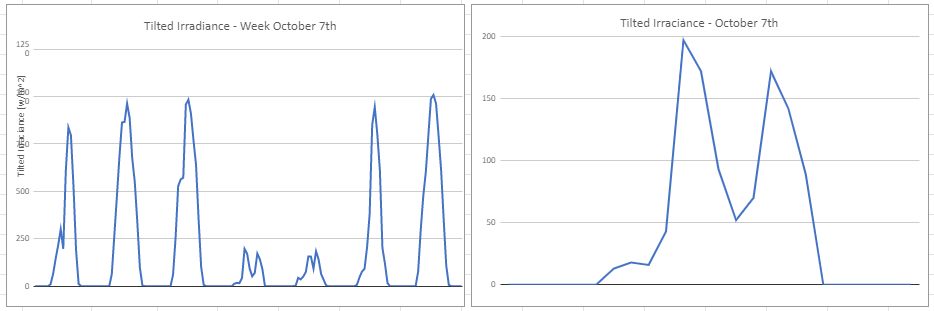
\includegraphics[width=0.5\textwidth]{inc/irr.png}
        \caption{Solar View tilted irradiance}
        \label{fig:solarview}
    \end{center}
\end{figure}

The historical data of track location, shows that on the day (October $7^{th}$) there is an expectation of significantly less nominal solar energy available. As shown \ref{fig:solarview} above the data expects a max of $200 W{\cdot}m^{-2}$ with significant midday dips. From this we can infer the very real possiblty of heavy/intermittent cloud cover.

\begin{table}[h!]
    \begin{center}
        \begin{tabular}{|l|l|}
            \hline
            \multicolumn{2}{|c|}{\textbf{Average Irr race period 11:00 - 14:00}} \\ \hline
            \textit{Oct 7th}                   & \textit{Week}                   \\ \hline
            96.75                              & 612.61                          \\ \hline
        \end{tabular}
    \end{center}
\end{table}

To prevent drastically oversizing the final design and to ensure optimising for total costing of the system, we examined the average irradiance over the race time of both the week as a whole and of the day itself (see above). From this we proceeded forth with expectation that the panels may be operating at half their possible maximum output. This directly informed the amount of panels we chose in order to supply our energy requirements, especially due to possible large fluctuation erring on a robust rather than exactly matched system.

\subsection{Topology}

\begin{center}
    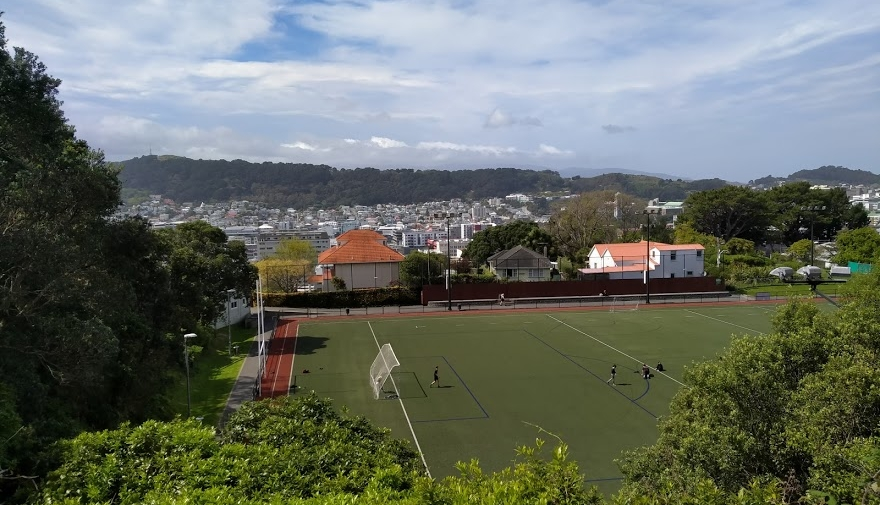
\includegraphics[width=0.5\textwidth]{inc/IMG20201006120746.jpg}
\end{center}

By visiting the site during the time on the week off the race, we were able to make an inspection of effects of shadows from building and trees. Seen above, the tree coverage of the northern tree line does not infringe on the section of field intended for solar collection, nor do any building. Therefore we can directly use the NIWA data under assumption that the only occlusion of direct sun we would experience would be cloud coverage.

\section{Race/Track Conditions}
\subsection{Description}
\begin{figure}[h!]
    \begin{center}
        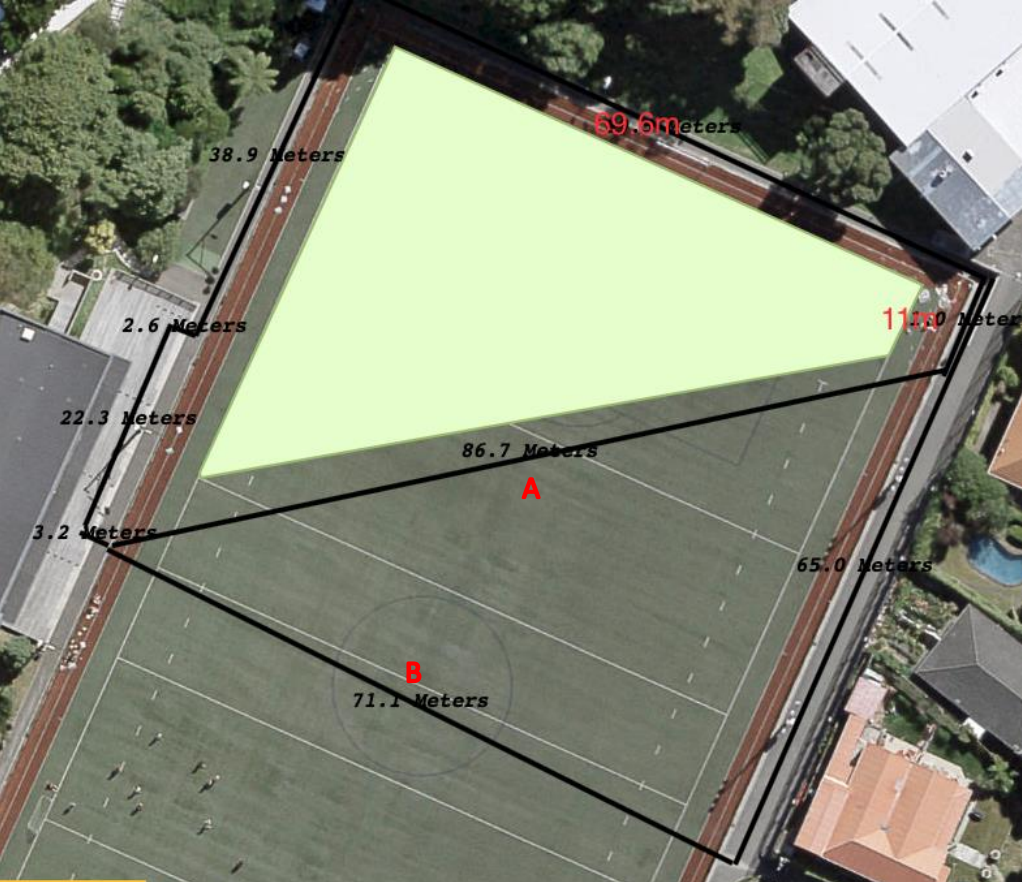
\includegraphics[width=0.42\textwidth]{inc/tracks.png}
        \caption{Track Options \cite{DANNYB}}
        \label{fig:routes}
    \end{center}
\end{figure}

The track as established consisted of two distinct course routes that were required to be chosen between. These are illustrated above [\ref{fig:routes}]: 

The first route, A, is roughly 234.3 meters and is roughly triangular.

The second , B, is $\approx 283.7$ meters but has the \textbf{possible} benefit of less distance on the turf.

The assumption that is required to be tested is that the current requirements of the 2 surface is of significant difference, ie higher on turf. Thus leading to a possible requirement of comparing trade off in potentially higher current draw to a shorter track.

\subsection{Testing}
To investigate the potential difference in motor performance, the testing procedure was to take one motor as a reference and perform set tasks while collected real-time data of current drawn from the battery.

We did this only for one motor to make observation to compare not necessarily the difference in motors but the general affect of surface and action on the power requirements of the platform.

\begin{figure}[h!]
    \begin{center}
        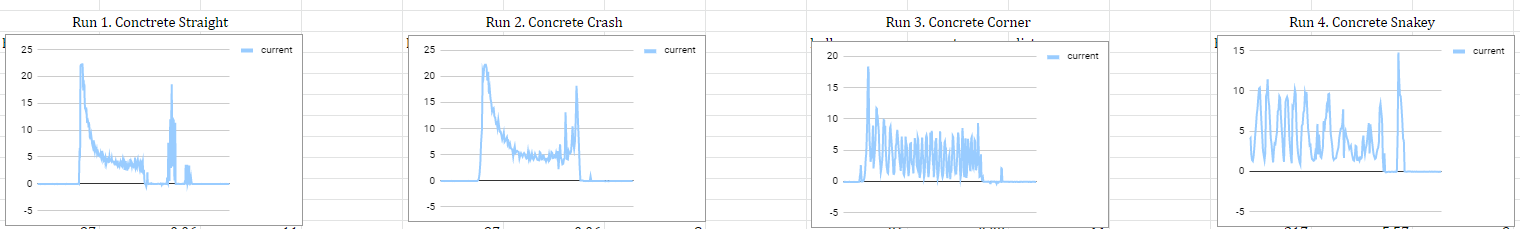
\includegraphics[width=\textwidth]{inc/contrete_behaviour.png}
        \caption{Concrete Performance}
        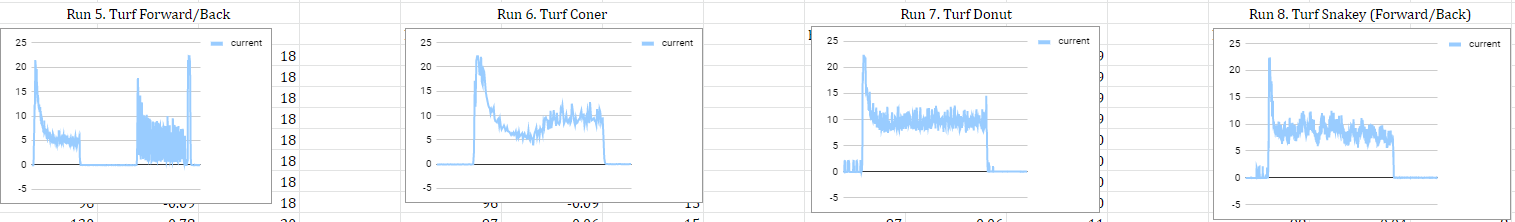
\includegraphics[width=\textwidth]{inc/turf_behaviour.png}
        \caption{Turf Performance}
    \end{center}
\end{figure}

We performed taking corners, from stand still acceleration and continuous turning on both surfaces build enough of an idea to compare.

From the data visualised above we observed a greater baseline current usage on the turf than the concrete, a significant up to 50\% greater current draw at times.

Behaviourally, it was observed that large acceleration spikes are consistent between the two surfaces, but due to the higher baseline of the turf the average current draw from alot of turning and corner taking draw more current, more consistently.\\

Using this initial analysis, we concluded that being in more control of the car to increase the time at straight, constant speed and reduce accelerations would most likely increase the lifetime of the battery charge and that the trade off between reduced length and higher current draw would have to be further examined and made up for with other optimisations.



\section{Component Testing}
\subsection{Motors}
To characterise and compare available motor types and performance a testing 

\begin{figure}[h!]
    \begin{center}
        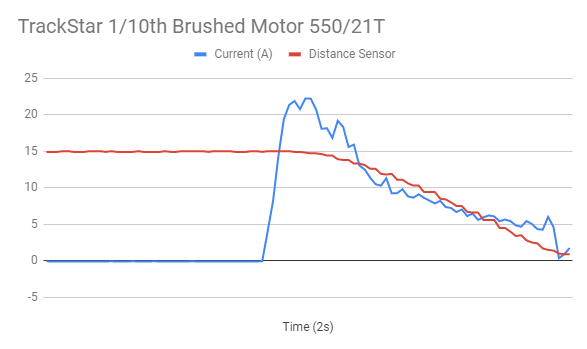
\includegraphics[width=0.3\textwidth]{inc/large_motor.png}
        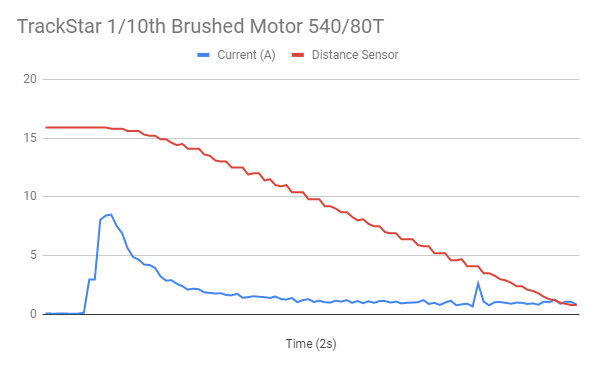
\includegraphics[width=0.3\textwidth]{inc/slow_motor.png}
        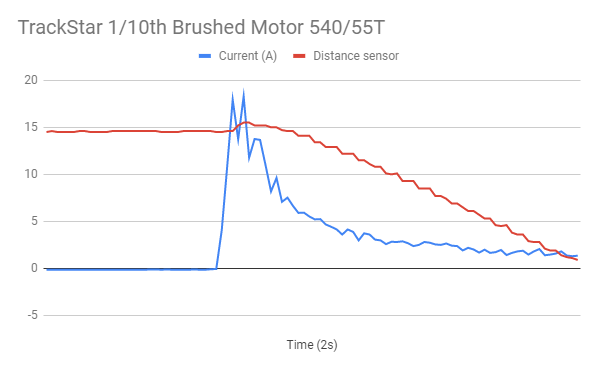
\includegraphics[width=0.3\textwidth]{inc/small_motor.png}
    \end{center}
\end{figure}

\subsection{Battery Capacity and Charge Time}

\section{System Design}
\subsection{Charge Station}

\begin{center}
    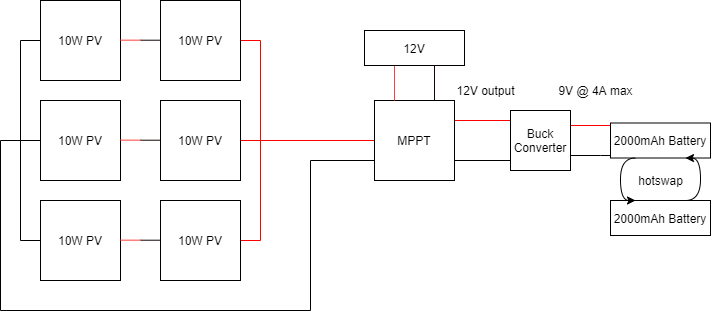
\includegraphics[width=0.5\textwidth]{inc/panels.png}
\end{center}

\subsection{Car}
\begin{figure}[h!]
    \begin{center}
        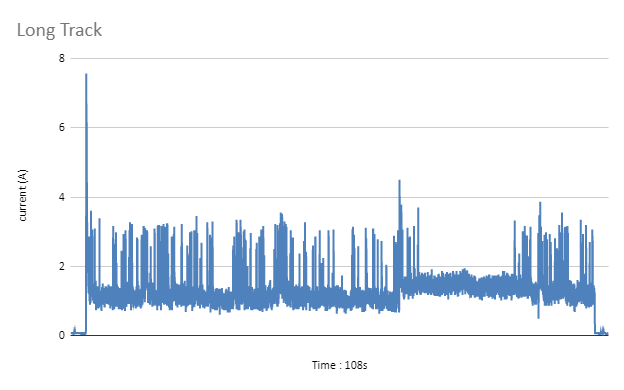
\includegraphics[width=0.3\textwidth]{inc/long_lap.png}
        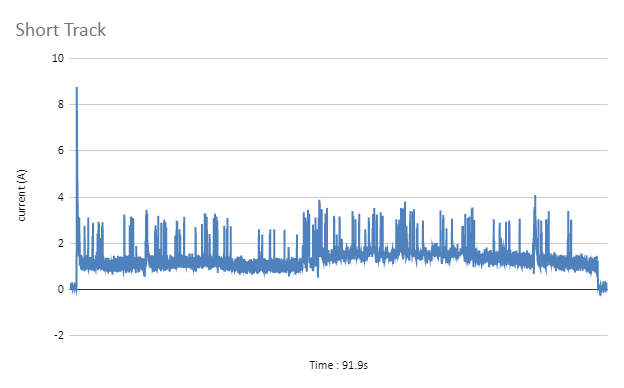
\includegraphics[width=0.3\textwidth]{inc/short_lap.png}
    \end{center}
\end{figure}
\section{Risk Analysis}

\section{Budget}

\begin{table}[h!]
    \begin{center}        
    \begin{tabular}{|l|l|}
    \hline
    \multicolumn{2}{|c|}{\textbf{Team ECO Budget}}            \\ \hline
    6 x 12V 10W Polycrystalline solar panel & 285.42 \\ \hline
    buck                                    & 12.39  \\ \hline
    MPPT + 12V bat                          & 86.85  \\ \hline
    2 x NiMH battery 2000mAh                & 154.44 \\ \hline
    TrackStar 1/10th Brushed Motor 540/80T  & 14.04  \\ \hline
    \textbf{total}                          & \textbf{553.14} \\ \hline
    \end{tabular}
    \end{center}
    \end{table}
\section{Conclusion}

\bibliography{ref}
\bibliographystyle{IEEEtran}
\end{document}
